%===============================================================================
\chapter{Identifica��o de controladores n�o lineares utilizando refer�ncia virtual}
\label{chapter:dbnarmax}
%===============================================================================

Este cap�tulo apresenta a uni�o das ideias de refer�ncia virtual para projetos de controladores e algoritmos de
identifica��o de sistemas n�o lineares.

No Cap�tulo \ref{chapter:nlin_si_ident} apresentou-se diversas estruturas de classes de modelos e em especial a
estrutura de modelos NARMAX, com suas representa��es polinomiais e racionais. Foi apresentado tamb�m (Se��o
\ref{sec:nl_si_algorithms_rationals}) um algoritmo para identifica��o deste tipo de classe de modelos. Naquele cap�tulo
deu-se �nfase ao uso deste algoritmo para identifica��o de sistemas n�o lineares. Na Se��o \ref{sec:dbnarmax_method}
ser� apresentado o uso deste algoritmo para identifica��o de controladores.

Para gerar os sinais de entrada e sa�da do algoritmo de identifica��o NARMAX, ser� utilizada a ideia de refer�ncia
virtual, introduzida na Se��o \ref{sec:dbcd_vrft} com o m�todo VRFT.

Ser�o apresentados na Se��o \ref{sec:dbnarmax_nonlinear_examples} alguns resultados obtidos com a metodologia proposta.
Os exemplos t�m o objetivo de cobrir as situa��es mais corriqueiras para identifica��o de controladores n�o lineares
NARMAX al�m de prover os resultados para que possa ser validada a usabilidade do m�todo.

%===============================================================================
%===============================================================================
\section{Introdu��o}
\label{sec:dbnarmax_intro}
%===============================================================================

Projeto de controladores descrito no Cap�tulo \ref{chapter:dbcd} tem como base a identifica��o de controladores
lineares. Encontram-se poucos trabalhos na literatura que abordam identifica��o de controladores n�o lineares baseados
nos dados coletados da planta. Em \cite{Guardabassi} � apresentado um procedimento para lineariza��o de sistemas n�o
lineares utilizando a ideia de refer�ncia virtual. Em \cite{campi_savaresi2006} � apresentada uma generaliza��o do
m�todo VRFT que envolve a identifica��o de controladores n�o lineares. Seguindo nesta linha, existem diversos trabalhos
propondo metodologias e algoritmos para a identifica��o de sistemas n�o lineares para in�meras fam�lias de modelos. Em
\cite{chen_billings1989Prediction} � apresentado uma metodologia para a estimativa de par�metros de sistemas n�o
lineares, de forma recursiva. Os mesmos autores no mesmo ano apresentaram um trabalho sobre identifica��o de sistemas
n�o lineares utilizando classes de modelos NARMAX \cite{chen_billings1989}. Em \cite{Hjalmarsson2012} � apresentada uma
modelagem de ordem finita de um modelo Hammerstein e sua acuracidade, modelagem esta que serve como refer�ncia para
parte do desenvolvimento que ser� apresentado na Se��o \ref{sec:dbnarmax_wiener_hammerstein}.

Existem na literatura diversos tipos de aplica��es para o conceito de refer�ncia virtual, para projeto de controladores
baseados em dados, o m�todo VRFT � talvez o mais conhecido. Neste trabalho tem-se o intuito de, baseado em refer�ncia
virtual, determinar os sinais de entrada para a utiliza��o de algum algoritmo de identifica��o de sistemas n�o
lineares, para com isso determinar qual � o controlador �timo para que o sistema se comporte em malha fechada como
desejado.


%===============================================================================
\section{Defini��es}
\label{sec:dbnarmax_defines}
%===============================================================================

No Cap�tulo \ref{chapter:system_identification} foram apresentadas as defini��es para identifica��o de sistemas
lineares. Definiu-se o sistema real pelo simbolo $\mathcal{S}$, para este cap�tulo $\mathcal{S}$ � um sistema n�o liner,
e para o projeto de controladores, o controlador ideal � definido por $\mathcal{C}_d$, sendo o controlador que consegue
fazer com que o sistema em malha fechada se comporte como desejado.

Define-se a classe de controladores n�o lineares como 

\begin{equation}
\mathcal{C}(\theta)
\label{eq:dbnarmax_controller_class}
\end{equation}

Diz-se que o controlador ideal pode ser representado pela classe de modelos, ou seja, $\mathcal{C}_d \in
\mathcal{C}(\theta)$, se existir um valor de $\theta_0$ que fa�a com que:

\begin{equation}
\mathcal{C}(\theta_0) = \mathcal{C}_d
\end{equation}

%===============================================================================
\section{M�todo}
\label{sec:dbnarmax_method}
%===============================================================================

O m�todo proposto consiste na ideia de utilizar refer�ncia virtual para, a partir dos dados coletados do
sistema, determinar os sinais de entrada do controlador que fazem com que o sistema em malha fechada se comporte como
desejado: $T_d(z)$.

Parte-se do pressuposto de que o processo $\mathcal{S}$ � n�o linear, mas que o comportamento em malha fechada
desejado $T_d(z)$ seja linear, portanto o controlador projetado deve, al�m de cumprir com os objetivos de performance
determinados, cancelar as n�o linearidades da planta para que possa ser poss�vel uma rela��o linear entre a entrada
$r(t)$ e a sa�da $y(t)$.

An�logamente ao que foi apresentado na Se��o \ref{sec:dbcd_vrft_framework} para controladores lineares, o controlador
n�o linear $\mathcal{C}(\theta)$  quando operando em conjnto com o sistema n�o linear $\mathcal{S}$ resulta um sistema
em malha fechada cuja fun��o de transfer�ncia � dada por $T_d(z)$. Obta-se que este comportamento em malha fechada seja
linear. Desta forma, se $T_d(z)$ for excitado com qualquer sinal $r(t)$, sua sa�da ser� $T_d(z)r(t)$. Uma premissa para
que o sistema em malha fechada tenha a mesma fun��o de transfer�ncia que o modelo de refer�ncia � que a sa�da dos dois
sejam a mesma para um dado sinal $\bar{r}(t)$.

Baseado no sinal $y(t)$ medido da sa�da do processo, considera-se um sinal $\bar{r}(t)$ tal que 
$T_d(z)\bar{r}(t)=y(t)$. Esta refer�ncia, como j� foi apresentada, � conhecida como {\it{virtual}} pois ela n�o existe e
n�o foi utilizada para gerar o sinal $y(t)$. A Figura \ref{fig:dbnarmax_method_vr} apresenta o sistema em malha fechada e
os sinais presentes.

\begin{figure}[htbp]
\center
% Generated with LaTeXDraw 2.0.8
% Wed Aug 01 22:46:20 BRT 2012
% \usepackage[usenames,dvipsnames]{pstricks}
% \usepackage{epsfig}
% \usepackage{pst-grad} % For gradients
% \usepackage{pst-plot} % For axes
\scalebox{1} % Change this value to rescale the drawing.
{
\begin{pspicture}(0,-1.4292188)(9.601875,1.4692189)
\pscircle[linewidth=0.04,linestyle=dashed,dash=0.16cm 0.16cm,dimen=outer](1.981875,0.97078127){0.2}
\psframe[linewidth=0.04,linestyle=dashed,dash=0.16cm 0.16cm,dimen=outer](5.381875,1.3707813)(3.581875,0.57078123)
\psframe[linewidth=0.04,dimen=outer](8.181875,1.3707813)(6.581875,0.57078123)
\psline[linewidth=0.04cm,arrowsize=0.05291667cm 2.0,arrowlength=1.4,arrowinset=0.4]{->}(0.581875,0.97078127)(1.781875,0.97078127)
\psline[linewidth=0.04cm,linestyle=dashed,dash=0.16cm 0.16cm,arrowsize=0.05291667cm 2.0,arrowlength=1.4,arrowinset=0.4]{->}(2.181875,0.97078127)(3.581875,0.97078127)
\psline[linewidth=0.04cm,arrowsize=0.05291667cm 2.0,arrowlength=1.4,arrowinset=0.4]{->}(5.381875,0.97078127)(6.581875,0.97078127)
\psline[linewidth=0.04cm](8.181875,0.97078127)(9.581875,0.97078127)
\psline[linewidth=0.04cm,linestyle=dashed,dash=0.16cm 0.16cm,arrowsize=0.05291667cm 2.0,arrowlength=1.4,arrowinset=0.4]{<-}(1.981875,0.7707813)(1.981875,-0.02921875)
\psline[linewidth=0.04cm,linestyle=dashed,dash=0.16cm 0.16cm](1.981875,-0.02921875)(8.981875,-0.02921875)
\psline[linewidth=0.04cm,linestyle=dashed,dash=0.16cm 0.16cm](8.981875,-0.02921875)(8.981875,0.97078127)
\usefont{T1}{ptm}{m}{n}
\rput(1.6198437,1.2807813){+}
\usefont{T1}{ptm}{m}{n}
\rput(2.1839063,0.68078125){-}
\usefont{T1}{ptm}{m}{n}
\rput(0.991875,1.2707813){\small $\bar{r}(t)$}
\usefont{T1}{ptm}{m}{n}
\rput(4.451875,0.97078127){\small $\mathcal{C}(\theta)$}
\usefont{T1}{ptm}{m}{n}
\rput(7.341875,0.9907812){\small $\mathcal{S}$}
\usefont{T1}{ptm}{m}{n}
\rput(6.031875,1.2707813){\small $u(t)$}
\usefont{T1}{ptm}{m}{n}
\rput(2.771875,1.2707813){\small $\epsilon (t)$}
\usefont{T1}{ptm}{m}{n}
\rput(8.821875,1.2707813){\small $y(t)$}
\psframe[linewidth=0.04,dimen=outer](6.581875,-0.62921876)(4.381875,-1.4292188)
\usefont{T1}{ptm}{m}{n}
\rput(5.431875,-1.0492188){\small $T_d^{-1}(z)$}
\psline[linewidth=0.04cm](9.581875,0.97078127)(9.581875,-1.0292188)
\psline[linewidth=0.04cm,arrowsize=0.05291667cm 2.0,arrowlength=1.4,arrowinset=0.4]{->}(9.581875,-1.0292188)(6.581875,-1.0292188)
\psline[linewidth=0.04cm](4.381875,-1.0292188)(0.581875,-1.0292188)
\psline[linewidth=0.04cm](0.581875,-1.0292188)(0.581875,0.97078127)
\end{pspicture} 
}
\caption{Representa��o em blocos do sistema em malha fechada para obten��o dos sinais $\epsilon(t)$ e $\bar{r}(t)$
utilizando refer�ncia virtual. Tracejado est� a realimenta��o e o controlador, que n�o est�o presentes no procedimento
para obten��o dos sinais.}
\label{fig:dbnarmax_method_vr}
\end{figure}

O sinal $\epsilon(t)$ � o erro entre os sinais $y(t)$ e $\bar{r}(t)$. Sabe-se que quando a planta �
excitada com o sinal $u(t)$, o sinal $y(t)$ � ent�o obtido. Analogamente para um controlador, quando este �
excitado com o sinal $\epsilon(t)$, o sinal $u(t)$ � obtido. A metodologia proposta, analogamente ao m�todo VRFT
consiste em encontrar um controlador, com os sinais $u(t)$ e $\epsilon(t)$ que s�o conhecidos, a tarefa ent�o reduz-se a
um problema de identifica��o de sistemas n�o lineares.

Fica a crit�rio do projetista, assim como para m�todos lineares, determinar a estrutura da classe de modelos a ser
utilizada para a identifica��o do controlador. Para que o comportamento linear $T_d(z)$ possa ser obtido
em malha fechada h� a necessidade de que o controlador $\mathcal{C}_d \in \mathcal{C}(\theta)$. 

N�o � apenas devido a planta ser n�o linear e o comportamento em malha fechada ser linear que o controlador ideal
possuir� um comportamento n�o linear. Pode-se a partir de um comportamento em malha fechada n�o linear e com uma planta
linear, ou n�o, obter-se um controlador que tamb�m seja n�o linear, dependendo das especifica��es que ao qual
o controlador � submetido.

%===============================================================================
\subsection{Classe do modelo}
\label{sec:dbnarmax_classes}
%===============================================================================

A escolha da classe de modelos $\mathcal{C}(\theta)$ que ir� representar o controlador ideal $\mathcal{C}_d$ � de grande
import�ncia para que haja sucesso no processo de identifica��o deste controlador. Neste trabalho optou-se pelo uso da
classe de modelos NARMAX apresentada na Se��o \ref{sec:nl_models_narmax} pela abrang�ncia desta classe de modelos em
representar sistemas reais e pelos bons resultados obtidos na identifica��o de sistemas n�o lineares apresentados na
Se��o \ref{sec:nl_si_algorithms_rationals_examples}.

Como foi apresentao, a classe de modelos NARMAX pode ser dividida em polinomial:

\begin{equation}
y(t)=\sum_{m=0}^{l}\sum_{p=0}^{m}\sum_{n1, n_m}^{n_y, n_u}c_{p,m-p}(n_1,...,n_m)\prod_{i=1}^{p}y(t-n_i)\prod_{i=p+1}^{m}u(t-n_i)
\nonumber
\end{equation}
e racional:

\begin{align*}
y(t) &=\frac{a(y(t-1), \ldots, y(t-n_y), u(t-1),\ldots, u(t-n_u), }{b(y(t-1), \ldots, y(t-n_y), u(t-1), \ldots, u(t-n_u),}\cdots \\ 
& \cdots\frac{ e(t-1), \ldots, e(t-n_e))}{e(t-1), \ldots, e(t-n_e))} +e(t)
\end{align*}

Aplica-se ent�o o algoritmo proposto na Se��o \ref{sec:nl_si_algorithms_rationals} para a identifica��o do controlador
$\mathcal{C}(\theta)$.

� conveniente observar que a escolha da classe NARMAX est� intimamente ligada ao uso do algoritmo de identifica��o
destes modelos ter-se mostrado bastante eficiente, como foi apresentado nos exemplos da Se��o
\ref{sec:nl_si_algorithms_rationals_examples}, al�m dos motivos j� citados da vasta gama de sistemas reais que modelos
NARMAX conseguem representar. Todavia, a metodologia apresentada, poderia ser aplicada para qualquer classe de modelos
de sistemas n�o lineares, onde algum algoritmo para identifica��o deste tipo de classe pudesse ser utilizado para
obten��o dos valores de $\hat{\theta}$ que minimizem algum crit�rio de escolha. Uma das poucas limita��es seria que este
algoritmo deveria identificar o controlador baseado nos dados de entrada e sa�da da planta e dos sinais virtuais gerados
a partir destes dados.

A qualidade das estimativas obtidas � bastante relacionada com a qualidade do algoritmo em estimar os valores de
$\theta$ que minimizam alguma fun��o custo. Entretanto tudo que foi abordado referente a identificabilidade de um
experimento e a ordem de excita��o de um sinal, determinam as condi��es b�sicas para que o resultado obtido seja livre
de erro de polariza��o.




%===============================================================================
\section{Wiener / Hammerstein}
\label{sec:dbnarmax_wiener_hammerstein}
%===============================================================================

Nesta se��o ser�o apresentados os resultados obtidos e os procedimentos para a identifica��o de controladores n�o
lineares modelados por uma classe de modelos polinomiais quando a planta $\mathcal{S}_{nl}$ � um sistema do tipo Wiener,
descritos na Se��o \ref{sec:nl_models_wiener_hammerstein}. Ser� utilizado o conceito de refer�ncia virtual para a
obten��o dos sinais necess�rios para que o projeto de identifica��o deste controlador possa ser realizado.

Considere que o sistema real possui uma n�o linearidade est�tica do tipo Wiener, onde o bloco n�o linear
encontra-se na sa�da do processo. Como descrito em:

\begin{eqnarray}
z(t) & = & G_0(q) u(t) + H_0 (q) e(t) \label{eq:wiener_z} \\
y(t) & = & \phi( z(t)) \label{eq:wiener_y}
\end{eqnarray}
onde $G_0(z)$ e $H_0(z)$ s�o fun��es de transfer�ncia racionais e o mapa  $\phi(\cdot ):
{\cal D}\rightarrow \cal D$, com $\cal D\subset \Re$, � analitico. A Figura \ref{fig:Wiener} representa este sismtea.

\begin{figure}[htbp]
\center
% Generated with LaTeXDraw 2.0.8
% Tue Sep 04 00:22:08 BRT 2012
% \usepackage[usenames,dvipsnames]{pstricks}
% \usepackage{epsfig}
% \usepackage{pst-grad} % For gradients
% \usepackage{pst-plot} % For axes
\scalebox{1} % Change this value to rescale the drawing.
{
\begin{pspicture}(0,-1.0367187)(6.8690624,1.0767188)
\pscircle[linewidth=0.04,dimen=outer](3.17,-0.63671875){0.2}
\psline[linewidth=0.04cm,arrowsize=0.05291667cm 2.0,arrowlength=1.4,arrowinset=0.4]{->}(0.37,-0.63671875)(1.17,-0.63671875)
\psframe[linewidth=0.04,dimen=outer](2.37,-0.23671874)(1.17,-1.0367187)
\psline[linewidth=0.04cm,arrowsize=0.05291667cm 2.0,arrowlength=1.4,arrowinset=0.4]{->}(3.37,-0.63671875)(4.37,-0.63671875)
\psframe[linewidth=0.04,dimen=outer](5.57,-0.23671874)(4.37,-1.0367187)
\psline[linewidth=0.04cm,arrowsize=0.05291667cm 2.0,arrowlength=1.4,arrowinset=0.4]{->}(2.37,-0.63671875)(2.97,-0.63671875)
\psline[linewidth=0.04cm,arrowsize=0.05291667cm 2.0,arrowlength=1.4,arrowinset=0.4]{->}(5.57,-0.63671875)(6.37,-0.63671875)
\usefont{T1}{ppl}{m}{n}
\rput(3.7245312,-0.32671875){$z(t)$}
\usefont{T1}{ppl}{m}{n}
\rput(0.48453125,-0.32671875){$u(t)$}
\usefont{T1}{ppl}{m}{n}
\rput(6.284531,-0.32671875){$y(t)$}
\usefont{T1}{ppl}{m}{n}
\rput(4.934531,-0.62671876){$\phi(\cdot)$}
\usefont{T1}{ppl}{m}{n}
\rput(1.7345313,-0.62671876){$G_0(q)$}
\psline[linewidth=0.04cm,arrowsize=0.05291667cm 2.0,arrowlength=1.4,arrowinset=0.4]{->}(0.37,0.56328124)(1.17,0.56328124)
\psframe[linewidth=0.04,dimen=outer](2.37,0.9632813)(1.17,0.16328125)
\psline[linewidth=0.04cm](2.37,0.56328124)(3.17,0.56328124)
\usefont{T1}{ppl}{m}{n}
\rput(0.48453125,0.87328124){$e(t)$}
\usefont{T1}{ppl}{m}{n}
\rput(1.7345313,0.59328127){$H_0(q)$}
\psline[linewidth=0.04cm,arrowsize=0.05291667cm 2.0,arrowlength=1.4,arrowinset=0.4]{->}(3.17,0.56328124)(3.17,-0.43671876)
\end{pspicture} 
}
\caption{Um sistema do tipo Wiener como descrito por \eqref{eq:wiener_z} e \eqref{eq:wiener_y}}
\label{fig:Wiener}
\end{figure}

Al�m disso � assumido que o mapa $\phi(\cdot )$ � invers�vel em todo range $\cal D$, ou seja, existe um mapa
$\phi_R^{-1}(\cdot )$ tal que $\phi(\phi_R^{-1}(x)) = x \quad \forall x \in {\cal D}$.

N�o � dificil de perceber que para este caso o controlador ideal � um sistema Hammerstein, ou seja:

\begin{eqnarray}
u(t) & = & C_d'(z) v(t)  \label{eq:hammer_u}\\
v(t) & = & r(t) - \psi( y(t) )\label{eq:hammer_v}
\end{eqnarray}

\begin{figure}[htbp]
\center
% Generated with LaTeXDraw 2.0.8
% Sun Sep 02 10:59:53 BRT 2012
% \usepackage[usenames,dvipsnames]{pstricks}
% \usepackage{epsfig}
% \usepackage{pst-grad} % For gradients
% \usepackage{pst-plot} % For axes
\scalebox{1} % Change this value to rescale the drawing.
{
\begin{pspicture}(0,-1.0367187)(4.6990623,1.0767188)
\pscircle[linewidth=0.04,dimen=outer](1.2,0.56328124){0.2}
\psline[linewidth=0.04cm,arrowsize=0.05291667cm 2.0,arrowlength=1.4,arrowinset=0.4]{->}(0.0,0.56328124)(1.0,0.56328124)
\psline[linewidth=0.04cm,arrowsize=0.05291667cm 2.0,arrowlength=1.4,arrowinset=0.4]{->}(1.4,0.56328124)(2.2,0.56328124)
\psframe[linewidth=0.04,dimen=outer](3.4,0.9632813)(2.2,0.16328125)
\psline[linewidth=0.04cm](1.2,-0.63671875)(2.2,-0.63671875)
\psframe[linewidth=0.04,dimen=outer](3.4,-0.23671874)(2.2,-1.0367187)
\psline[linewidth=0.04cm,arrowsize=0.05291667cm 2.0,arrowlength=1.4,arrowinset=0.4]{->}(1.2,-0.63671875)(1.2,0.36328125)
\psline[linewidth=0.04cm,arrowsize=0.05291667cm 2.0,arrowlength=1.4,arrowinset=0.4]{->}(3.4,0.56328124)(4.2,0.56328124)
\psline[linewidth=0.04cm,arrowsize=0.05291667cm 2.0,arrowlength=1.4,arrowinset=0.4]{<-}(3.4,-0.63671875)(4.2,-0.63671875)
\usefont{T1}{ptm}{m}{n}
\rput(0.48453125,0.87328124){$r(t)$}
\usefont{T1}{ptm}{m}{n}
\rput(4.114531,0.87328124){$u(t)$}
\usefont{T1}{ptm}{m}{n}
\rput(4.114531,-0.32671875){$y(t)$}
\usefont{T1}{ptm}{m}{n}
\rput(1.7145313,0.87328124){$v(t)$}
\usefont{T1}{ptm}{m}{n}
\rput(2.7645311,-0.62671876){$\psi(\cdot)$}
\usefont{T1}{ptm}{m}{n}
\rput(2.7745314,0.5732812){$C_d'(z)$}
\psline[linewidth=0.04cm](1.38,0.34328124)(1.54,0.34328124)
\end{pspicture} 
}
\caption{Um controlador do tipo Hammerstein como descrito por \eqref{eq:hammer_u} e \eqref{eq:hammer_v}}
\label{fig:dbnarmax_method_vr}
\end{figure}

Realmente, se $\psi(\cdot ) = \phi_R^{-1}(\cdot )$ e 
\begin{equation}
C_d' (q)= \frac{T_d(q)}{G_0(q)(1-T_d(q))}
\label{eq:dbcd_perf_tracking_cd}
\end{equation}

Ent�o o sismtema em malha fechada � linear com uma fun��o de transfer�ncia $T_d(q)$.

Na pr�tica esta � uma solu��o padr�o de controle, pois controladores comerciais normalmente incluen customiz�veis
fun��es de lineariza��o  $\psi(\cdot )$  no la�o de realimenta��o. Fica claro que nesmo neste caso padr�o o controlador
ideal n�o � uma fun��o do erro de refer�ncia $r(t)-y(t)$, mas sim uma fun��o de  $r(t)$ e de $y(t)$ separadamente. 

Assumindo que a refer�ncia � uma constante conhecida, uma topologia alternativa pode ser elaborada com um controlador
que � dependente apenas do erro de refer�ncia. A classe de modelos deste controlador pode ser definido como:

\begin{eqnarray}
u(t) & = & C'(z,\rho) v(t) \label{eq:track_error_controller_u}\\
v(t) & = & \psi( r(t) - y(t),\eta )\label{eq:track_error_controller_v}
\end{eqnarray}
onde a fun��o $\psi(\cdot,\cdot )$ deve ser tal que o sistema com o controlador em malha fechada deveria se comportar
como se nenhuma das n�o linearidades estivesse presente, ou seja:

\begin{equation}
\psi ( r(t) - y(t) ) = \alpha [r(t)-z(t)]
\label{vzlinear}
\end{equation}
para algum $\alpha\in\Re^+$. A Figura \ref{fig:vrft_nl_wiener} mostra um sistema com uma n�o linearidade do tipo
Wiener e um controlador descrito como anteriormente.

\begin{figure}[htbp]
\center
% Generated with LaTeXDraw 2.0.8
% Sat Aug 25 13:00:53 BRT 2012
% \usepackage[usenames,dvipsnames]{pstricks}
% \usepackage{epsfig}
% \usepackage{pst-grad} % For gradients
% \usepackage{pst-plot} % For axes
\scalebox{0.95} % Change this value to rescale the drawing.
{
\begin{pspicture}(0,-2.12)(12.480156,2.1)
\psline[linewidth=0.04cm,arrowsize=0.05291667cm 2.0,arrowlength=1.4,arrowinset=0.4]{->}(0.0471875,0.3)(1.0471874,0.3)
\pscircle[linewidth=0.04,dimen=outer](1.2471875,0.3){0.2}
\psline[linewidth=0.04cm,arrowsize=0.05291667cm 2.0,arrowlength=1.4,arrowinset=0.4]{->}(1.4471874,0.3)(2.36,0.3)
\psframe[linewidth=0.04,dimen=outer](3.56,0.7)(2.36,-0.1)
\psline[linewidth=0.04cm,arrowsize=0.05291667cm 2.0,arrowlength=1.4,arrowinset=0.4]{->}(3.56,0.3)(4.36,0.3)
\psframe[linewidth=0.04,dimen=outer](5.56,0.7)(4.36,-0.1)
\psframe[linewidth=0.04,dimen=outer](8.36,0.7)(7.16,-0.1)
\psframe[linewidth=0.04,dimen=outer](10.96,0.7)(9.76,-0.1)
\psline[linewidth=0.04cm,arrowsize=0.05291667cm 2.0,arrowlength=1.4,arrowinset=0.4]{->}(5.447188,0.3)(7.16,0.3)
\psline[linewidth=0.04cm,arrowsize=0.05291667cm 2.0,arrowlength=1.4,arrowinset=0.4]{<-}(1.2471875,0.1)(1.2471875,-2.1)
\psline[linewidth=0.04cm](1.2471875,-2.1)(11.56,-2.1)
\usefont{T1}{ppl}{m}{n}
\rput(0.45453125,0.61){$r(t)$}
\usefont{T1}{ppl}{m}{n}
\rput(1.5807812,0.61){$\epsilon (t)$}
\usefont{T1}{ppl}{m}{n}
\rput(3.930781,0.57){$v(t)$}
\usefont{T1}{ppl}{m}{n}
\rput(6.365625,0.61){$u(t)$}
\usefont{T1}{ppl}{m}{n}
\rput(9.460782,0.61){$z(t)$}
\usefont{T1}{ppl}{m}{n}
\rput(11.895625,0.61){$y(t)$}
\psline[linewidth=0.04cm](1.4671875,0.08)(1.6671875,0.08)
\psframe[linewidth=0.04,linestyle=dashed,dash=0.16cm 0.16cm,dimen=outer](5.96,1.3)(1.96,-0.7)
\psframe[linewidth=0.04,linestyle=dashed,dash=0.16cm 0.16cm,dimen=outer](11.36,2.1)(6.76,-0.7)
\usefont{T1}{ppl}{m}{n}
\rput(3.950781,-0.99){$\mathcal{C}$}
\usefont{T1}{ppl}{m}{n}
\rput(8.870782,-0.99){$\mathcal{S}$}
\usefont{T1}{ppl}{m}{n}
\rput(2.9207811,0.31){$\psi(\cdot)$}
\usefont{T1}{ppl}{m}{n}
\rput(10.320781,0.31){$\phi(\cdot)$}
\usefont{T1}{ppl}{m}{n}
\rput(4.910781,0.31){$C'(q)$}
\usefont{T1}{ppl}{m}{n}
\rput(7.720781,0.31){$G_0(q)$}
\psframe[linewidth=0.04,dimen=outer](8.36,1.7)(7.16,0.9)
\usefont{T1}{ppl}{m}{n}
\rput(7.720781,1.29){$H_0(q)$}
\psline[linewidth=0.04cm](8.36,1.3)(8.96,1.3)
\psline[linewidth=0.04cm,arrowsize=0.05291667cm 2.0,arrowlength=1.4,arrowinset=0.4]{->}(8.96,1.3)(8.96,0.5)
\pscircle[linewidth=0.04,dimen=outer](8.96,0.3){0.2}
\psline[linewidth=0.04cm,arrowsize=0.05291667cm 2.0,arrowlength=1.4,arrowinset=0.4]{->}(8.36,0.3)(8.76,0.3)
\psline[linewidth=0.04cm,arrowsize=0.05291667cm 2.0,arrowlength=1.4,arrowinset=0.4]{->}(9.16,0.3)(9.76,0.3)
\psline[linewidth=0.04cm,arrowsize=0.05291667cm 2.0,arrowlength=1.4,arrowinset=0.4]{->}(6.36,1.3)(7.16,1.3)
\usefont{T1}{ppl}{m}{n}
\rput(6.285625,1.61){$e(t)$}
\psline[linewidth=0.04cm,arrowsize=0.05291667cm 2.0,arrowlength=1.4,arrowinset=0.4]{->}(10.96,0.3)(12.16,0.3)
\psline[linewidth=0.04cm](11.56,-2.1)(11.56,0.3)
\end{pspicture} 
}
\caption{Diagrama de blocos para um sistema n�o linear do tipo Wiener}
\label{fig:vrft_nl_wiener}
\end{figure}

Ao faz�-lo, o controlador ideal depende apenas do erro de refer�ncia, mas a fun��o  $\psi(\cdot )$ depende do valor de
refer�ncia, e ser� uma fun��o diferente para cada valor diferente da refer�ncia. Al�m disso, para valores n�o
constantes, a n�o linearidade inversa $\psi(\cdot)$ pode n�o ser autonoma, violando outra pressuposi��o da formula��o
n�o linear do VRFT proposta em \cite{campi_savaresi2006}.

Agora, entretanto � desejado que o sistem se comporte linearmente em malha fechada como $T_d(q)$. Para obter-se isso o
controlador deve cancelar todos os efeitos n�o lineares de $\phi(z(t))$. Em outras palavras, � desejado que em malha
fechada o sinal $v(t)$ obede�a a equa��o (\ref{vzlinear}). Entretanto o sistema apresentado na Figura
\ref{fig:vrft_nl_wiener} se comporta como em:

\begin{equation}
v(t)=\psi (r(t) - y(t))
\nonumber
\end{equation}
e assim podemos obter a rela��o entre $\psi(\cdot) $ e $\phi(\cdot)$ como:

\begin{equation}
\psi (r(t) - \phi(z(t))) = \alpha [r(t) - z(t)] .
\label{eq:dbnarmac_ex_wiener_psi}
\end{equation}

Fica claro que qunado n�o existe um sinal de refer�ncia, $r(t) \equiv 0$, a rela��o entre os polinomios $\psi(\cdot)$ e
$\phi(\cdot)$ fica simplificada a:

\begin{equation}
\psi (\phi(z(t))) = -\alpha z(t)
\nonumber 
\end{equation}
ent�o neste caso (mas apenas neste caso) $\psi(\cdot )$ deve ser a inversa de  $\phi(\cdot)$, a menos de uma
constante.

\subsection{Convexidade}

O ponto principal do paradigma de refer�ncia virtual � de deixar o problema de modelo de refer�ncia convexo. Isso �
obtido no VRFT por meio de uma parametriza��o linear do controlador e o projeto do controlador � obtido por meio da
solu��o de um problema de m�nimos quadrados.

The main point of the virtual reference paradigm is to convexify the model reference problem. This is
obtained in VRFT by means of a linear parameterization of the controller and the 
controller design is performed by the solution of a least squares problem.
A fim de aproveitar esta virtude computacional, � necessario ter um controlador parametrizavel linearmente. Desde que a
inversa � assumidamente analitica, ela pode ser espandida em serie de Taylor e ent�o truncada:

$$
\phi_R^{-1} ( x ) \cong  \sum_{i=0}^{k} \frac{1}{i!}\frac{\partial^i \phi_R^{-1} }{\partial x^i}( 0 ) x^i 
$$%\\ & \bydef & \sum_{i=0}^{k} \alpha_i x^i \eeqan

Se o controlador e a fun��o n�o linear forem ambos parametrizaveis linearmente, ou seja, 

\begin{eqnarray}
C'(z,\theta ) & = & \frac{1}{D(z)} \theta^T N(z) \label{um} \\
\psi(\epsilon(t)) & = & \eta^T E(t) \label{dois}
\end{eqnarray}
com $D(z)$ sendo um polinomio m�nico conhecido, $N(z)\bydef [1 \quad z^{-1} z^{-2} \ldots
z^{-p}]^T$, e $E(t) \bydef [\epsilon (t) \quad \epsilon^2 (t) \ldots \epsilon^k (t)]^T$.
Ent�o, definindo  $u_f(t) = D(z) u(t)$ e substituindo as equa��es \eqref{um} e \eqref{dois} em
\eqref{eq:hammer_u} leva a:

\begin{equation}
u_f(t) = \sum_{i=0}^{p} \sum_{j=1}^k \rho_{i+j} \epsilon^j(t-i)
\end{equation}
ou
\begin{equation}
u_f(t) = \rho^T \varpi(t)
\end{equation}
onde $\rho_{i+j} \bydef \theta_i\eta_j$ e o vetor $\rho=\left[ \rho_1 \ldots \rho_{pk}\right]^T$ s�o os par�metros a
serem identificados. Note que um pre�o precisa ser pago para se obter uma parametriza��o linear: o n�mero de parametros
que inicialmente era igual a $p+k$, � agora $p\times k$.

O exemplo num�rico abaixo visa demonstrar este m�todo proposto para o projeto de controladores do tipo Hammerstein.


%===============================================================================
\subsection{Exemplo num�rico}
\label{sec:dbnarmax_wiener_hammerstein_exemple}
%===============================================================================
 
Considere uma planta n�o linear $\mathcal{S}_{nl}$ do tipo Wiener como apresentado na Figura \ref{fig:vrft_nl_wiener}.
Considere ainda que o bloco linear desta planta pode ser descrito como abaixo:

\begin{equation}
G'(q)=\frac{0.5}{q-0.9}
\label{eq:vrft_nl_wiener_g}
\end{equation}
e a n�o linearidade presente na planta do sistema pode ser descrita como um polin�mio de terceira ordem:

\begin{equation}
\zeta(\omega(t))=y(t)=1.5\omega(t)+0.2\omega^3(t)
\label{eq:vrft_nl_wiener_zeta}
\end{equation}  
tem-se assim que a planta pode ser descrita pela concatena��o dos blocos $G'(q)$ e $\zeta(t)$.

A fun��o $\gamma(\cdot)$ foi previamente definida pela equa��o \eqref{eq:dbnarmac_ex_wiener_gamma} e por esta equa��o
n�o ser parametriz�vel por um modelo NARMAX devido a $\zeta(\cdot)$ apresentado em \eqref{eq:vrft_nl_wiener_zeta}, aproxima-se
$\gamma(\cdot)$ como abaixo:

\begin{equation}
\gamma (\epsilon(t))= v(t) = a_1\epsilon (t) + a_2 \epsilon ^2(t) +a_3 \epsilon ^3(t) +a_4 \epsilon ^4(t)
\label{eq:dbnarmax_ex_wiener_gamma_choosen}
\end{equation}  

Desta forma o controlador a ser identificado pode ser modelado por um modelo NARMAX, mesmo isso sendo uma aproxima��o do
controlador ideal $\mathcal{C}_d$. Desta forma n�o � poss�vel afirmar que $\mathcal{C}_d \in \mathcal{C}$. 

Considerando entretanto que nenhum dos blocos n�o lineares existissem no sistema, o controlador ideal poderia ser descrito pela equa��o
\eqref{eq:dbcd_perf_tracking_cd}, resultando em 

\begin{equation}
C_d'(q)= \frac{0.8q-0.72}{q-1}
\label{eq:vrft_nl_wiener_cd}
\end{equation}
entretanto, o controlador ideal que leva o sistema a se comportar como definido por $T_d(q)$ � composto em parte por
\eqref{eq:vrft_nl_wiener_cd} acrescido do polin�mio \eqref{eq:dbnarmax_ex_wiener_gamma_choosen}.

O controlador $C_d'(q)$ possui um integrador em sua estrutura. Para evitar problemas de seguimento de
refer�ncia optou-se por n�o identificar esta parte do controlador, mantendo o denominador como um integrador
e identificando apenas o numerador. 

Fazendo-se as substitui��es necess�rias, chega-se � express�o do sinal de sa�da do controlador que se quer identificar:

\begin{align}\nonumber
u(t) =&  \theta_1 \epsilon (t)+ \theta_2 \epsilon ^2(t)+ \theta_3 \epsilon^3(t)+ \theta_4 \epsilon^4(t)+\\
& \theta_5 \epsilon(t-1)+ \theta_6 \epsilon^2(t-1)+  \theta_7 \epsilon^3(t-1)+ \theta_8 \epsilon^4(t-1)
\label{eq:dbnarmax_ex_wiener_controller}
\end{align}

Observa-se que $u(t)$ em \eqref{eq:dbnarmax_ex_wiener_controller} � um modelo NARMAX polinomial. Foram realizados 100
experimentos de Monte Carlo adicionando um ru�do com $\sigma_e^2=0.05$ e utilizando o algoritmo para identifica��o de
modelos NARMAX em conjunto com o procedimento de refer�ncia virtual para gerar os sinais $r(t)$ e $\epsilon(t)$ e a
m�dia das estimativas obtidas foi de:

\begin{equation}
\theta_{\text{m�dia}} =\begin{bmatrix}
0.44717 \\ 2.0216\times10^{-3} \\ -6.5181\times10^{-4} \\ -1.608\times10^{-5} \\ -0.40435 \\ -1.6163\times10^{-3} \\
6.1265\times10^{-4}\\ 1.469\times10^{-5} 
\end{bmatrix}^T
\nonumber
\end{equation}
%com uma matriz de covari�ncia de:
%
%\begin{equation}
%\theta_{\text{Covari�ncia}} =\begin{bmatrix}
%5.2065e-06 & 	 -9.7986e-08 & 	 -1.9078e-08 & 	 -3.2055e-10 & 	 -3.6186e-06 & 	 1.2798e-07 & 	 5.9285e-09 & 	 -2.0474e-10  \\ 
%-9.7986e-08 & 	 5.5494e-08 & 	 -5.4726e-10 & 	 -1.5158e-10 & 	 1.0123e-07 & 	 -4.4708e-08 & 	 3.9962e-10 & 	 1.2237e-10  \\ 
%-1.9078e-08 & 	 -5.4726e-10 & 	 2.1459e-10 & 	 9.3647e-12 & 	 4.4485e-09 & 	 3.1849e-10 & 	 -2.5329e-11 & 	 -2.0593e-12  \\ 
%-3.2055e-10 & 	 -1.5158e-10 & 	 9.3647e-12 & 	 8.0071e-13 & 	 -1.9028e-10 & 	 8.5314e-11 & 	 -1.6175e-12 & 	 -2.9308e-13  \\ 
%-3.6186e-06 & 	 1.0123e-07 & 	 4.4485e-09 & 	 -1.9028e-10 & 	 5.0042e-06 & 	 -8.9899e-08 & 	 -1.6759e-08 & 	 -1.5359e-10  \\ 
%1.2798e-07 & 	 -4.4708e-08 & 	 3.1849e-10 & 	 8.5314e-11 & 	 -8.9899e-08 & 	 6.9081e-08 & 	 -7.8269e-10 & 	 -2.0938e-10  \\ 
%5.9285e-09 & 	 3.9962e-10 & 	 -2.5329e-11 & 	 -1.6175e-12 & 	 -1.6759e-08 & 	 -7.8269e-10 & 	 1.5274e-10 & 	 7.6667e-12  \\ 
%-2.0474e-10 & 	 1.2237e-10 & 	 -2.0593e-12 & 	 -2.9308e-13 & 	 -1.5359e-10 & 	 -2.0938e-10 & 	 7.6667e-12 & 	 9.0946e-13  \\ 
%\end{bmatrix}
%\nonumber
%\end{equation}


O custo obtido $J_{y}(\theta_{\text{m�dia}})=0.3820$ e o custo dos sinais de sa�da do controlador ($u(t)$) esperado e
obtido foi $J_{VR}(\theta_{\text{m�dia}}=1.0119$.

Como $\gamma(\cdot)$ escolhido em \eqref{eq:dbnarmax_ex_wiener_gamma_choosen} � apenas uma aproxima��o do que
esperava-se em \eqref{eq:dbnarmac_ex_wiener_gamma}, sabe-se que a classe de modelos escolhida para o controlador pode
n�o conseguir representar a totalidade das din�micas do controlador ideal $\mathcal{C}_d$. Desta forma � esperado que
a identifica��o n�o consiga atingir a totalidade da fun��o $T_d(q)$ inicialmente escolhida. Para as estimativas foram
utilizados sinais de entrada do tipo PRBS com 127 pontos para a excita��o da planta.

Na Figura \ref{fig:vrft_nl_wiener_step} � apresentado um comparativo entre o sinal de sa�da do sistema
$T_d(q)$ quando submetido a um degrau unit�rio e o sinal do sistema real quando o controlador identificado com
$\theta_{\text{m�dio}}$ � aplicado sobre a planta em malha fechada.

\begin{figure}[htbp] 
	\center 
	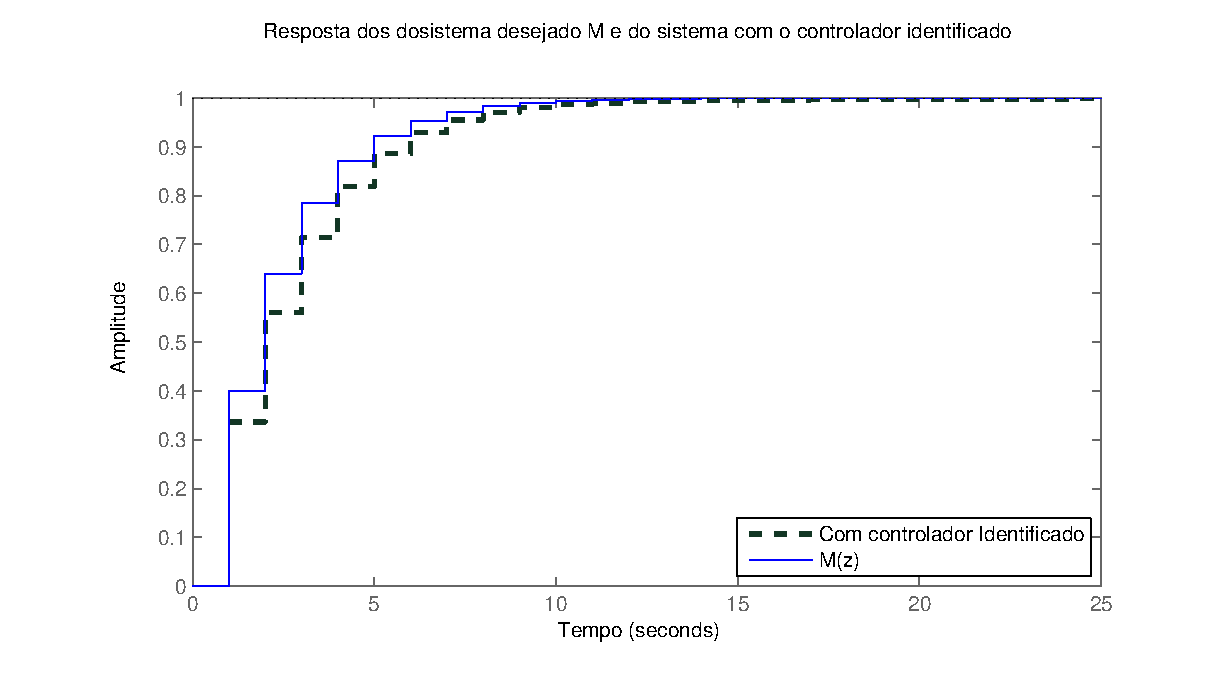
\includegraphics[width=0.95\columnwidth]{figures/vrft_nl_wiener_step.eps}
	\caption{Comparativo da resposta a um degrau unit�rio do modelo de refer�ncia $T_d(q)$ com o sistema real quando o
	controlador n�o linear representado por um modelo NARMAX polinomial � inserido na planta.}
	\label{fig:vrft_nl_wiener_step}
\end{figure}

Na Figura \ref{fig:vrft_nl_wiener_vw_step} � apresentado o comportamento dos sinais de sa�da e entrada das
n�o linearidades $\gamma(\epsilon(t))$ e $\zeta(\omega(t))$ respectivamente.

\begin{figure}[htbp] 
	\center 
	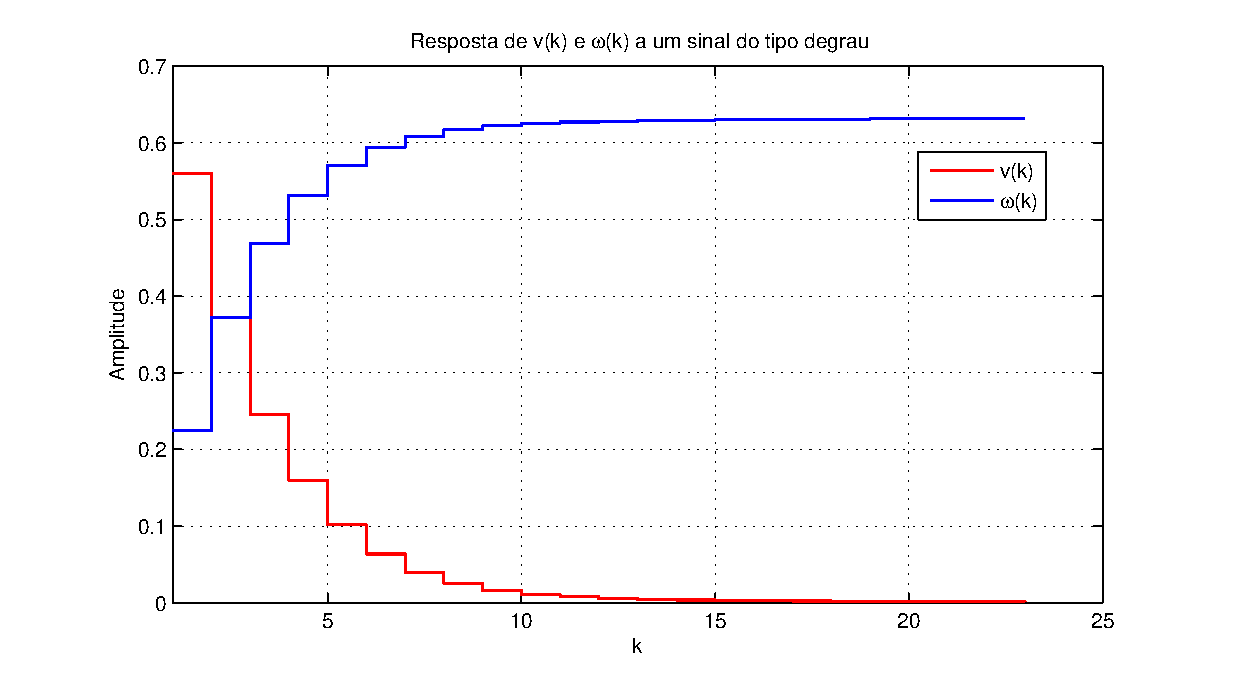
\includegraphics[width=0.95\columnwidth]{figures/vrft_nl_wiener_vw_step.eps}
	\caption{Sinais $v(t)$ e $\omega(t)$ do sistema apresentado na Figura \ref{fig:vrft_nl_wiener} quando este �
	excitado por um degrau unit�rio.}
	\label{fig:vrft_nl_wiener_vw_step}
\end{figure}

A rela��o entre os sinais $v(t)$ e $\omega(t)$ � apresentado na Figura \ref{fig:vrft_nl_wiener_vw}.
Observa-se que a rela��o destes sinais � afim, garantido desta forma que a aproxima��o feita em
\eqref{eq:dbnarmax_ex_wiener_gamma_choosen} foi suficiente para representar com acuracidade o que era esperado para
$\gamma(t)$ em \eqref{eq:dbnarmac_ex_wiener_gamma}.

\begin{figure}[htbp] 
	\center 
	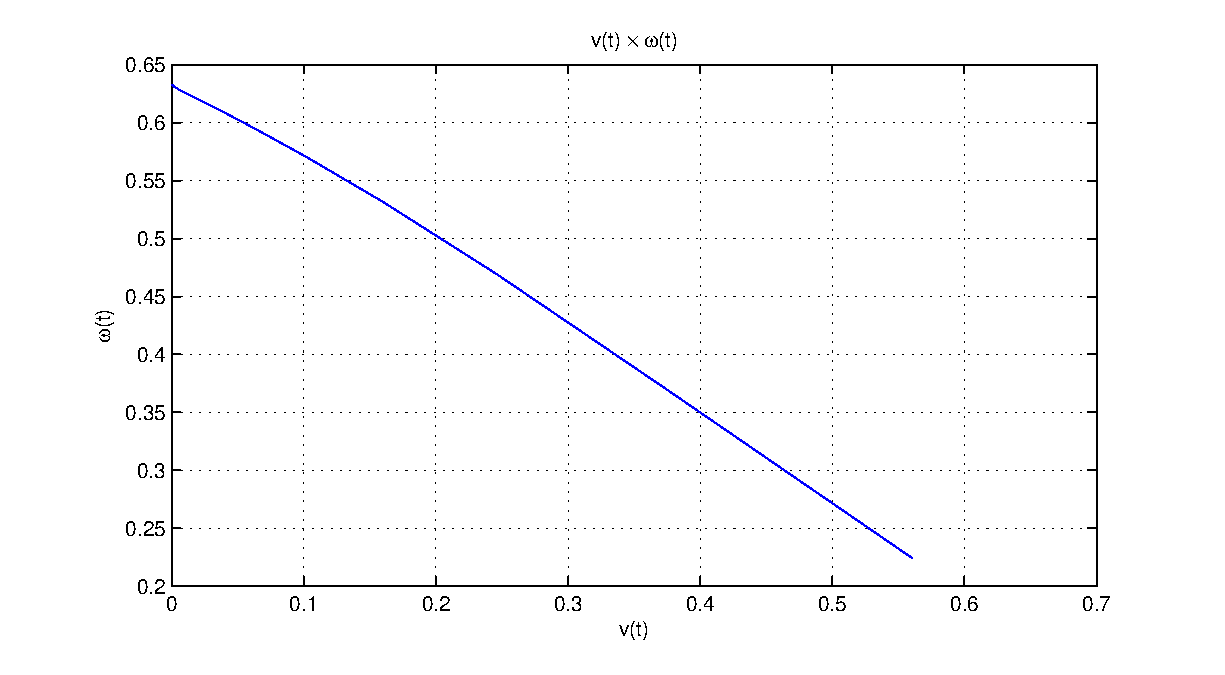
\includegraphics[width=0.95\columnwidth]{figures/vrft_nl_wiener_vw.eps}
	\caption{Rela��o entre os sinais $v(t)$ e $\omega(t)$ quando o sistema � alimentado por um degrau unit�rio}
	\label{fig:vrft_nl_wiener_vw}
\end{figure}


% ===============================================================================
\section{Exemplos ilustrativos}
\label{sec:dbnarmax_nonlinear_examples}
%===============================================================================

Neste trabalho o foco est� em apresentar os resultados da identifica��o de sistemas que podem ser descritos por modelos
NARMAX racionais ou polinomiais. Sendo que para isso ser�o apresentados exemplos de identifica��o de sistemas onde a
linearidade � est�tica assim como quando a n�o linearidade est� na din�mica do sistema.

Nos exemplos abordados a seguir as n�o linearidades estar�o presentes na planta do sistema e deseja-se que este sistema
se comporte em malha fechada como um sistema linear. Para isso o controlador adicionado na malha dever� ser capaz de
anular a n�o linearidade contida na planta, desta forma, for�ozamente o controlador ser� n�o linear, sendo descrito por
um modelo NARMAX racional ou polinomial.

Os exemplos apresentados a seguir s�o divididos em duas categorias: uma delas onde a n�o linearidade da planta est�
acoplada de forma est�tica e outra quando a n�o linearidade est� na din�mica do processo.

%===============================================================================
\subsection{N�o linearidades est�ticas}
\label{sec:dbnarmax_nl_wiener}
%===============================================================================

A planta do sistema utilizada neste exemplo possui uma n�o linearidade est�tica do tipo Wiener, onde o bloco n�o linear
encontra-se na sa�da do processo. Na Figura \ref{fig:vrft_nl_wiener} � apresentado o diagrama de blocos do sistema,
sendo $\zeta(t)$ e $\gamma(t)$ os blocos n�o lineares da planta e do controlador respectivamente. An�logamente
$G'(z)$ e $C'(z)$ s�o os blocos lineares da planta e do controlador. Como a n�o linearidade do controlador est� na
entrda deste, pode ser caracterizado como uma classe de Hammerstein, mas ser� identificado por uma classe de modelos
NARMAX racional.

\begin{figure}[htbp]
\center
% Generated with LaTeXDraw 2.0.8
% Sat Jun 16 14:47:44 BRT 2012
% \usepackage[usenames,dvipsnames]{pstricks}
% \usepackage{epsfig}
% \usepackage{pst-grad} % For gradients
% \usepackage{pst-plot} % For axes
\scalebox{1} % Change this value to rescale the drawing.
{
\begin{pspicture}(0,-1.72)(13.22,1.7)
\psline[linewidth=0.04cm,arrowsize=0.05291667cm 2.0,arrowlength=1.4,arrowinset=0.4]{->}(0.0,0.7)(1.0,0.7)
\pscircle[linewidth=0.04,dimen=outer](1.2,0.7){0.2}
\psline[linewidth=0.04cm,arrowsize=0.05291667cm 2.0,arrowlength=1.4,arrowinset=0.4]{->}(1.4,0.7)(2.8,0.7)
\psframe[linewidth=0.04,dimen=outer](4.0,1.1)(2.8,0.3)
\psline[linewidth=0.04cm,arrowsize=0.05291667cm 2.0,arrowlength=1.4,arrowinset=0.4]{->}(4.0,0.7)(5.0,0.7)
\psframe[linewidth=0.04,dimen=outer](6.2,1.1)(5.0,0.3)
\psframe[linewidth=0.04,dimen=outer](9.2,1.1)(8.0,0.3)
\psline[linewidth=0.04cm,arrowsize=0.05291667cm 2.0,arrowlength=1.4,arrowinset=0.4]{->}(9.2,0.7)(10.2,0.7)
\psframe[linewidth=0.04,dimen=outer](11.4,1.1)(10.2,0.3)
\psline[linewidth=0.04cm,arrowsize=0.05291667cm 2.0,arrowlength=1.4,arrowinset=0.4]{->}(6.2,0.7)(8.0,0.7)
\psline[linewidth=0.04cm,arrowsize=0.05291667cm 2.0,arrowlength=1.4,arrowinset=0.4]{->}(11.4,0.7)(13.2,0.7)
\psline[linewidth=0.04cm,arrowsize=0.05291667cm 2.0,arrowlength=1.4,arrowinset=0.4]{<-}(1.2,0.5)(1.2,-1.7)
\psline[linewidth=0.04cm](1.2,-1.7)(12.4,-1.7)
\psline[linewidth=0.04cm](12.4,-1.7)(12.4,0.7)
\usefont{T1}{ppl}{m}{n}
\rput(0.45828125,1.01){$r(t)$}
\usefont{T1}{ppl}{m}{n}
\rput(1.9445312,1.01){$\epsilon (t)$}
\usefont{T1}{ppl}{m}{n}
\rput(4.514531,1.01){$v(t)$}
\usefont{T1}{ppl}{m}{n}
\rput(7.089375,1.01){$u(t)$}
\usefont{T1}{ppl}{m}{n}
\rput(9.664532,1.01){$\omega(t)$}
\usefont{T1}{ppl}{m}{n}
\rput(12.499375,1.01){$y(t)$}
\psline[linewidth=0.04cm](1.6,0.5)(1.8,0.5)
\psframe[linewidth=0.04,linestyle=dashed,dash=0.16cm 0.16cm,dimen=outer](6.6,1.7)(2.4,-0.3)
\psframe[linewidth=0.04,linestyle=dashed,dash=0.16cm 0.16cm,dimen=outer](11.8,1.7)(7.6,-0.3)
\usefont{T1}{ppl}{m}{n}
\rput(4.3345313,-0.59){C(z)}
\usefont{T1}{ppl}{m}{n}
\rput(9.744532,-0.59){G(z)}
\usefont{T1}{ppl}{m}{n}
\rput(3.3945312,0.69){$\gamma(t)$}
\usefont{T1}{ppl}{m}{n}
\rput(10.794531,0.71){$\zeta(t)$}
\usefont{T1}{ppl}{m}{n}
\rput(5.594531,0.71){C'(z)}
\usefont{T1}{ppl}{m}{n}
\rput(8.604531,0.71){G'(z)}
\end{pspicture} 
}

\caption{Diagrama de blocos para um sistema n�o linear do tipo Wiener}
\label{fig:vrft_nl_wiener}
\end{figure}

O sistema possui um boloco linear que pode ser descrito por:

\begin{equation}
G'(z)=\frac{0.5}{z-0.9}
\label{eq:vrft_nl_wiener_g}
\end{equation} 

O comportamento do sistema em malha fechada esperado � definido por $M(z)$:

\begin{equation}
M(z)=\frac{0.4}{z-0.6}
\label{eq:vrft_nl_wiener_m}
\end{equation}  

A n�o linearidade presente na planta do sistema foi escolhida como sendo um polin�mio de terceira ordem
descrito como abaixo:

\begin{equation}
\zeta(\omega(t))=y(t)=1.5\omega(t)+0.2\omega^3(t)
\label{eq:vrft_nl_wiener_phi}
\end{equation}  

Espera-se ent�o que por $M(z)$ ser linear, que o controlador tenha um bloco que cancele o efeito n�o linear de
$\zeta(t)$.

Deseja-se que em malha fechada o sinal $v(t)$ seja tal que:

\begin{equation}
v(t)=r(t)-\omega(t)
\end{equation}

Tem-se entretanto:

\begin{equation}
v(t)=\epsilon(t)\gamma (t)
\nonumber
\end{equation}

e que

\begin{equation}
\epsilon(t) = r(t) - y(t)
\nonumber
\end{equation}
 
Obtem-se ent�o o relacionamento entre os sinais $\gamma (t) $ e $\zeta(t)$:

\begin{equation}
( r(t) - \omega(t) \zeta(t)) \gamma (t) = r(t) - \omega(t) 
\nonumber
\end{equation}

Resultando:

\begin{equation}
\gamma (t) = \frac{r(t)-\omega(t)}{r(t) - \omega(t)\zeta(t)} 
\end{equation}

Pecebe-se claramente que quando n�o h� sinal de refer�ncia $r(t)$, o relacionamento entre os polinomios $\gamma (t) $
e $\zeta(t)$ fica simplificado a:

\begin{equation}
\gamma (t) = \frac{1}{\zeta(t)}
\nonumber 
\end{equation}

Define-se ent�o $\gamma (t)$ como sendo:

\begin{equation}
\gamma (\epsilon(t))= v(t) = a_1\epsilon (t) + a_2 \epsilon ^2(t) +a_3 \epsilon ^3(t) +a_4 \epsilon ^4(t)
\label{eq:vrft_nl_wiener_phi_inv}
\end{equation}  

Desconsiderando a parte n�o linear presente na planta, � simples de observar que o controlador �timo que
levaria a planta em malha fechada a ter o comportamento descrito por $M(z)$ �:

\begin{equation}
C_d(z)= \frac{0.8z-0.72}{z-1}
\label{eq:vrft_nl_wiener_cd}
\end{equation}  

O controlador $C_d(z)$ possui uma integrador em sua estrutura. Para evitar problemas de seguimento de
refer�ncia optou-se por n�o identificar esta parte do controlador. Mantendo o denominador como um integrador
e identificando apenas o numerador. Juntamente com a identifica��o do controlador da por��o linear $C_d(z)$ �
necess�rio identificar o polin�mio da equa��o \eqref{eq:vrft_nl_wiener_phi_inv}.

Fazendo-se as substitui��es matem�ticas necess�rias, chega-se a express�o do sinal de sa�da do controlador que
se quer identificar:

\begin{equation}
u(t)=\begin{bmatrix}
\theta_1 & \theta_2 & \theta_3 & \theta_4 & \theta_5 & \theta_6 & \theta_7 & \theta_8
\end{bmatrix}
\begin{bmatrix}
\epsilon (t)\\ 
\epsilon ^2(t)\\ 
\epsilon^3(t)\\ 
\epsilon^4(t)\\ 
\epsilon(t-1)\\ 
\epsilon^2(t-1)\\ 
\epsilon^3(t-1)\\ 
\epsilon^4(t-1)
\end{bmatrix}
\label{eq:vrft_nl_wiener_u}
\end{equation}  

Onserva-se que $u(t)$ em \eqref{eq:vrft_nl_wiener_u} � um modelo NARMAX polinomial. Foram realizados 100 experimentos
de Monte Carlo utilizando o algoritmo para identifica��o de modelos NARMAX em conjunto com o procedimento de refer�ncia
virtual para gerar os sinais $r(t)$ e $\epsilon(t)$ e a m�dia das estimativas obtidas foi de:

\begin{equation}
\text{m�dia }\;\theta =\begin{bmatrix}
0.4471 \\ 0.0020 \\ -6.5105\times10^{-4} \\ -1.5959\times10^{-5} \\ -0.4043 \\ -0.0016 \\ 6.1194\times10^{-4}
\\ 1.4562\times10^{-5}
\end{bmatrix}^T
\nonumber
\end{equation}

Com um desvio padr�o de:

\begin{equation}
\text{m�dia }\;\theta = 1\times10^{-3}\begin{bmatrix}
0.2430 \\ 0.0246 \\ 0.0015 \\ 0.0001 \\ 0.2613 \\ 0.0259 \\ 0.0016 \\ 0.0001
\end{bmatrix}^T
\nonumber
\end{equation}

O custo entre os sinais de sa�da do sistema obtido e o sistema esperado $M(z)$ foi de  $J_{MR}(\theta)=
0.3820$ e o custo dos sinais de sa�da do controlador ($u(t)$) esperado e obtido foi de $J_{VR}=1.0119$.

Como a estimativa de $\gamma (\epsilon(t))$ � apenas uma aproxima��o do que espera-se ser a inversa de
$\zeta(\omega(t))$, a classe de modelos escolhida para o controlador n�o consegue representar a totalidade do
controlador ideal. Desta forma � esperado que a identifica��o n�o consiga atingir a totalidade da fun��o
$M(z)$ inicialmente escolhida. Para as estimativas foram utilizados sinais de entrada do tipo PRBS com 127 pontos para a
excita��o da planta.

Na Figura (\ref{fig:vrft_nl_wiener_step}) � apresentado um comparativo entre o sinal de sa�da do sistema
$M(z)$ quando submetido a um degrau unit�rio e o sinal do sistema real quando o controlador identificado �
aplicado sobre a planta em malha fechada.

\begin{figure}[htbp] 
	\center 
	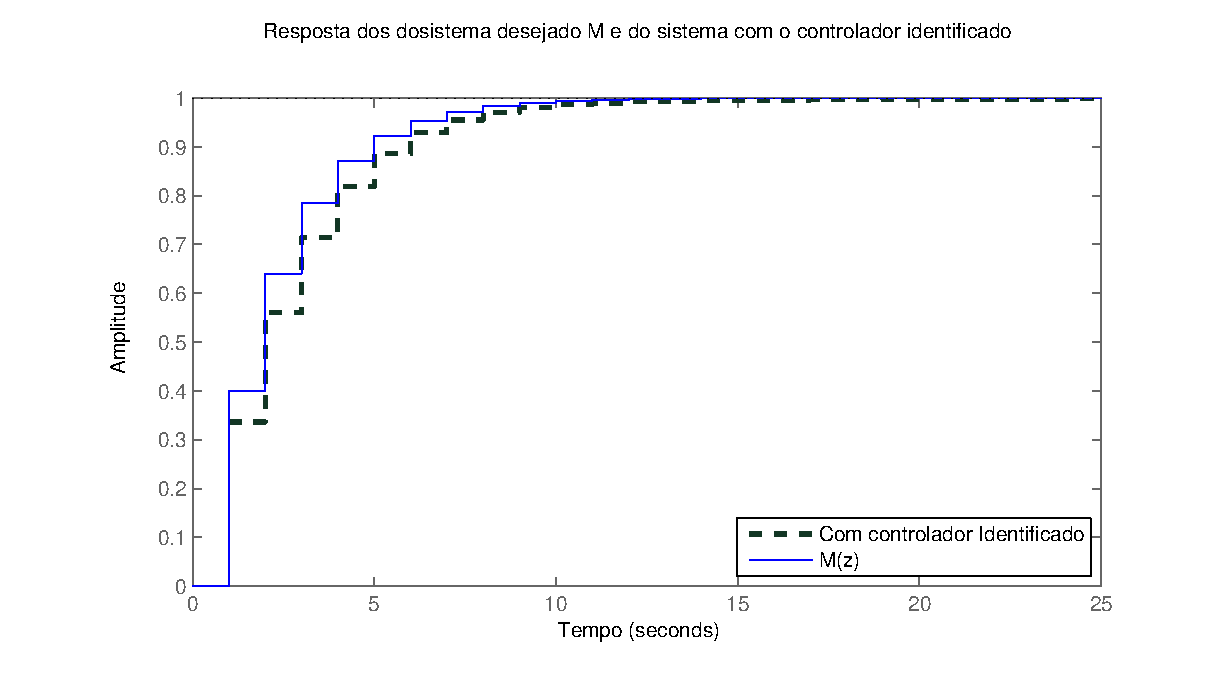
\includegraphics[width=0.95\columnwidth]{figures/vrft_nl_wiener_step.eps}
	\caption{resposta dos sistemas: desejado e obtido a um degrau unit�rio}
	\label{fig:vrft_nl_wiener_step}
\end{figure}

Na Figura (\ref{fig:vrft_nl_wiener_vw_step}) � apresentado o comportamento dos sinais de sa�da e entrada das
n�o linearidades $\gamma(\epsilon(t))$ e $\zeta(\omega(t))$ respectivamente.

\begin{figure}[htbp] 
	\center 
	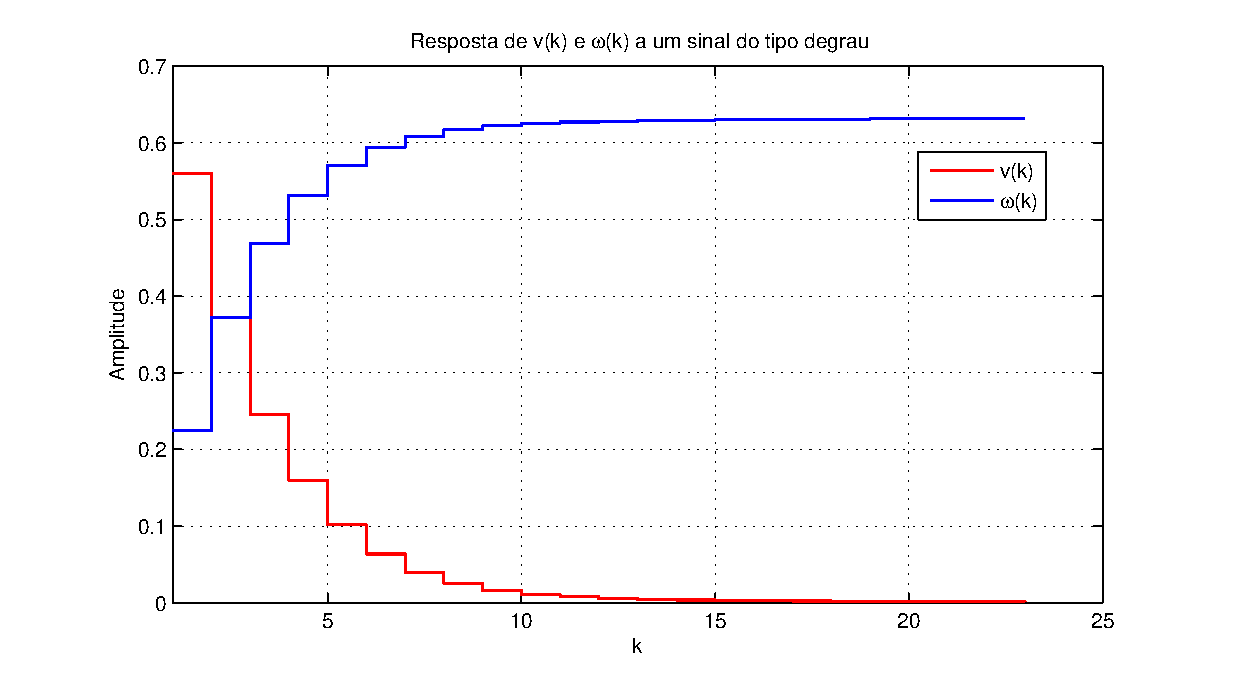
\includegraphics[width=0.95\columnwidth]{figures/vrft_nl_wiener_vw_step.eps}
	\caption{sinais $v(t)$ e $\omega(t)$ quando o sistema � alimentado por um degrau unit�rio}
	\label{fig:vrft_nl_wiener_vw_step}
\end{figure}

A rela��o entre os sinais $v(t)$ e $\omega(t)$ � apresentado na Figura (\ref{fig:vrft_nl_wiener_vw}).
Observa-se que a rela��o destes sinais � praticamente linear, garantido que a aproxima��o de $\gamma(\epsilon(t))$
foi satisfat�ria para representar a inversa do sinal $\zeta(\omega(t))$.

\begin{figure}[htbp] 
	\center 
	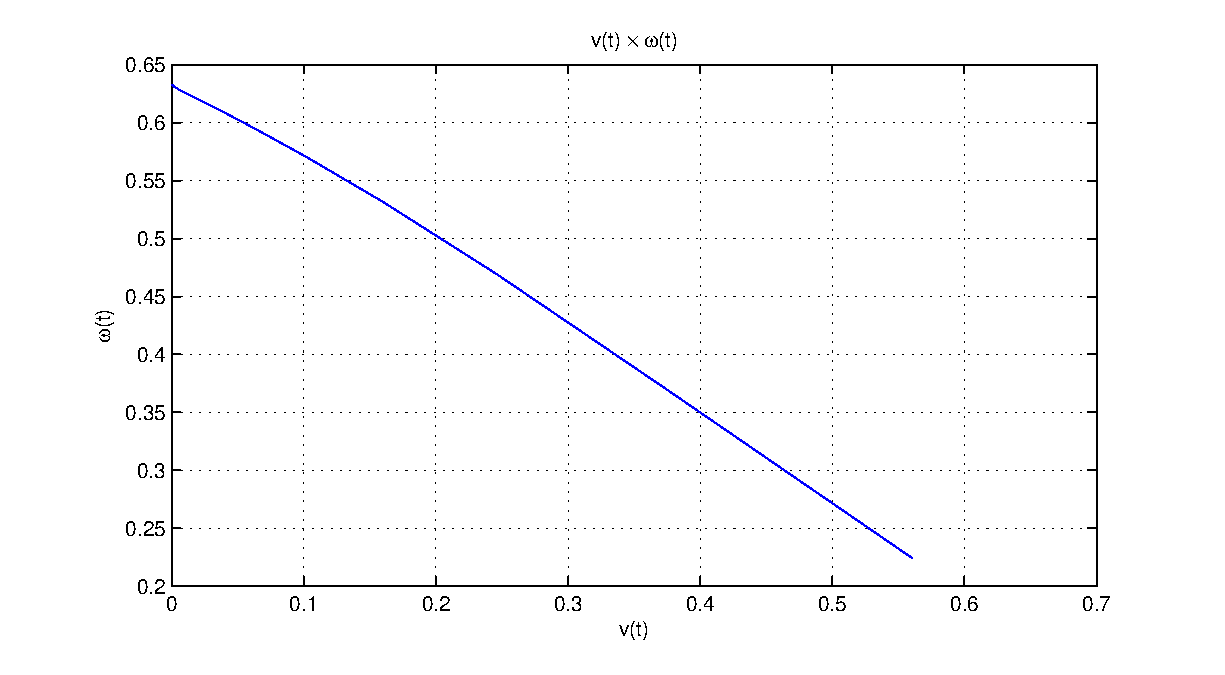
\includegraphics[width=0.95\columnwidth]{figures/vrft_nl_wiener_vw.eps}
	\caption{rela��o entre os sinais $v(t)$ e $\omega(t)$ quando o sistema � alimentado por um degrau unit�rio}
	\label{fig:vrft_nl_wiener_vw}
\end{figure}

%===============================================================================
\subsection{N�o linearidades din�micas}
\label{sec:dbnarmax_nl_dinamic}
%===============================================================================

Quando a n�o linearidade est� na din�mica do processo n�o h� uma distin��o entre um bloco linear e outro linear como
apresentado no exeplo anterior (se��o \ref{sec:dbnarmax_nl_wiener}). Ser�o apresentados aqui alguns exemplos de
identifica��o de controladores que podem ser representados por modelos NARMAX racionais.

Inicialmente um exemplo onde o controlador que leva a planta $G_0(z)$ a se comportar em malha fechada como em $M(z)$,
ser� totalmente representado pelo modelo escolhido para o controlador. Em seguida ser� apresentado para esta mesma
situa��o onde o controlador necess�rio � um pouco mais complexo, tendo mais vari�veis para identificar.

Ao fim ser� apresentado um exemplo onde o controlador ideal n�o consegue ser representado pela classe de modelos
escolhida.

Em todos os exemplos ser� utilizado para excitar o sistema, um sinal PRBS de ordem 7.

%===============================================================================
\subsubsection{Controlador ideal sendo representado pela classe de modelos}
\label{sec:dbnarmax_nl_dinamic_c_match}
%===============================================================================

Neste exemplo ser� abordado o caso onde o controlador $C(z, \theta) \in \mathcal{C}$. Fazendo com que o sistema em
malha fechada se comporte como desejado. Considere a planta n�o linear descrita por:

\begin{equation}
y(t)=\frac{0.5u(t-1)y(t-1)+u(t-1)}{1+0.25y^2(t-2)}
\label{eq:vrft_nl_dinamic_ex1_y}
\end{equation}

Deseja-se que em malha fechada seu comportamento seja linear como em:

\begin{equation}
M(z)=\frac{0.4}{z-0.6}
\label{eq:vrft_nl_dinamic_ex1_mz}
\end{equation}

A equa��o \eqref{eq:vrft_nl_dinamic_ex1_mz} pode ser reescrita em fun��o do tempo como em:

\begin{equation}
y(t)=0.4r(t-1)+0.6y(t-1)
\label{eq:vrft_nl_dinamic_ex1_mt}
\end{equation}

Ao igualar a equa��o \eqref{eq:vrft_nl_dinamic_ex1_y} com \eqref{eq:vrft_nl_dinamic_ex1_mt} e isolar o
sinal $u(t)$ tem-se a equa��o que descreve o comportamento do controlador que levar� a planta a ter o
comportamento descrito por $M(z)$ em malha fechada. Obt�m-se desta forma um controlador ideal como em:

\begin{equation}
u(t)=\frac{0.4r(t)+0.6y(t)+0.1y^2(t-1)r(t)+0.15y(t)y^2(t-1)}{1+0.5y(t)}
\label{eq:vrft_nl_dinamic_ex1_cd}
\end{equation}

Escolhendo uma classe de modelos que consegue representar o controlador �timo:

\begin{equation}
u(t)=\frac{\theta_1 r(t)+ \theta_2 y(t)+ \theta_3 y^2(t-1)r(t)+ \theta_4 y(t)y^2(t-1)}{1+ \theta_5 y(t)}
\label{eq:vrft_nl_dinamic_ex1_c}
\end{equation}

Utilizando um sinal PRBS de tamanho 254 pontos e o m�todo de refer�ncia virtual para gerar os sinais $r(t)$ e
$\epsilon(t)$. Adicionando-se um ruido de vari�ncia $\sigma^2 = 0.005$ a sa�da do sistema, a m�dia das estimativas para
100 experimentos de Monte Carlo foi de:

\begin{equation}
\theta_{\text{m�dia}}=\begin{bmatrix}
0.4000 & 0.5999 & 0.1001 & 0.1501 & 0.5000
\end{bmatrix}
\nonumber
\end{equation}

Os valores reais utilizados na simula��o foram:

\begin{equation}
\theta_0=\begin{bmatrix}
0.4 & 0.6 & 0.1 & 0.15 & 0.5
\end{bmatrix}
\nonumber
\end{equation} 

Obte-se um desvio padr�o para as estimativas de:

\begin{equation}
\theta_{\text{desvio padr�o}}=1.0\times 10^{-3}\begin{bmatrix}
0.2231 & 0.6866 & 0.2411 & 0.6817 & 0.3019
\end{bmatrix}
\nonumber
\end{equation}

A matriz de covari�ncia � descrita por:

\begin{equation}
\theta_{\text{Covari�ncia}}=1.0\times 10^{-6}\begin{bmatrix}
 0.0498 &  0.0585 & -0.0353 & -0.0362 & -0.0018 \\
 0.0585 &  0.4714 & -0.0449 & -0.3690 &  0.0057 \\
-0.0353 & -0.0449 &  0.0581 &  0.0745 & -0.0040 \\
-0.0362 & -0.3690 &  0.0745 &  0.4647 & -0.0070 \\
-0.0018 &  0.0057 & -0.0040 & -0.0070 &  0.0911
\end{bmatrix}
\nonumber
\end{equation}

Simulando o sistema com o controlador obtido pela m�dia das estimativas e o sistema em malha fechada
desejado, o erro observado para um sinal de entrada do tipo degrau unit�rio � apresentado na Figura
\ref{fig:vrft_nl_dynamic_step_erro}.

\begin{figure}[htbp] 
	\center 
	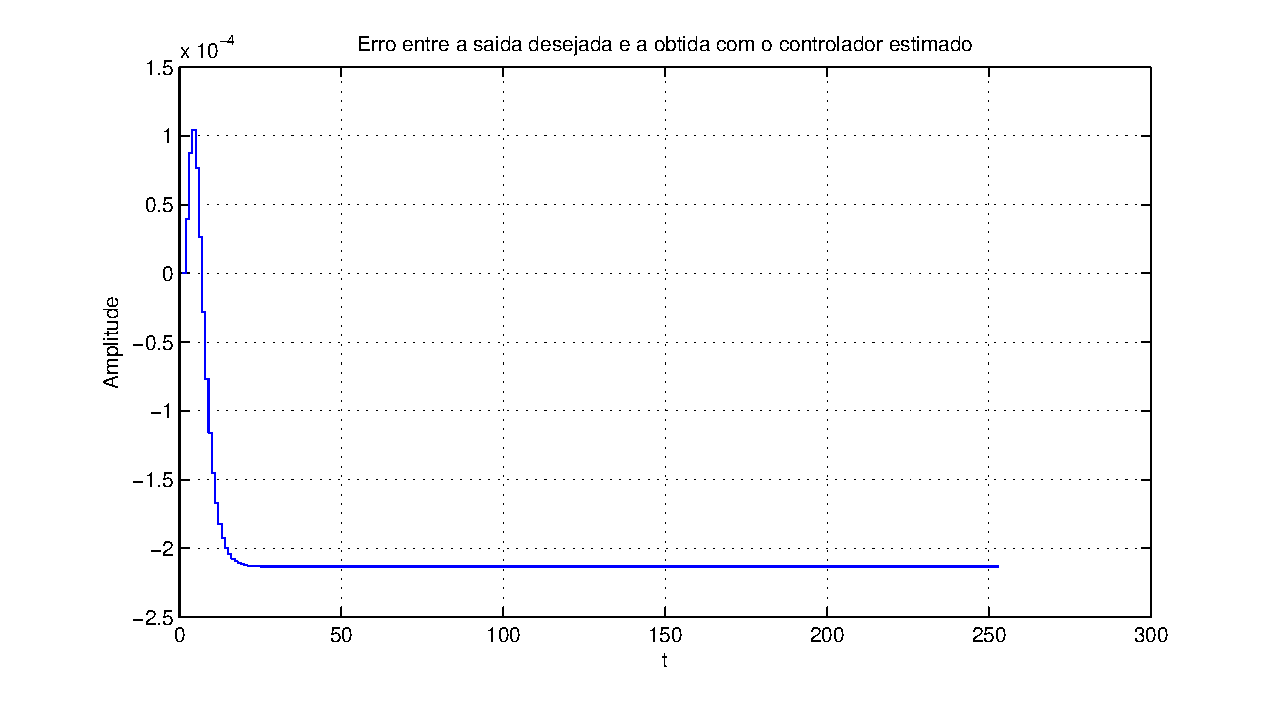
\includegraphics[width=0.95\columnwidth]{figures/vrft_nl_dynamic_erro_step.eps}
	\caption{Erro entre o a resposta esperada e obtida para uma entrada do tipo degrau unit�rio}
	\label{fig:vrft_nl_dynamic_step_erro}
\end{figure}

A fim de ilustrar as estimativas obtidas pelo m�todo, na Figura \ref{fig:vrft_nl_dynamic_t1_t2} s�o
apresentados as estimativas para os 100 experimentos realizados, al�m da elipse de confian�a de $\chi^2=95\%$
para os parametros $\theta_1$ e $\theta_2$.

\begin{figure}[htbp] 
	\center 
	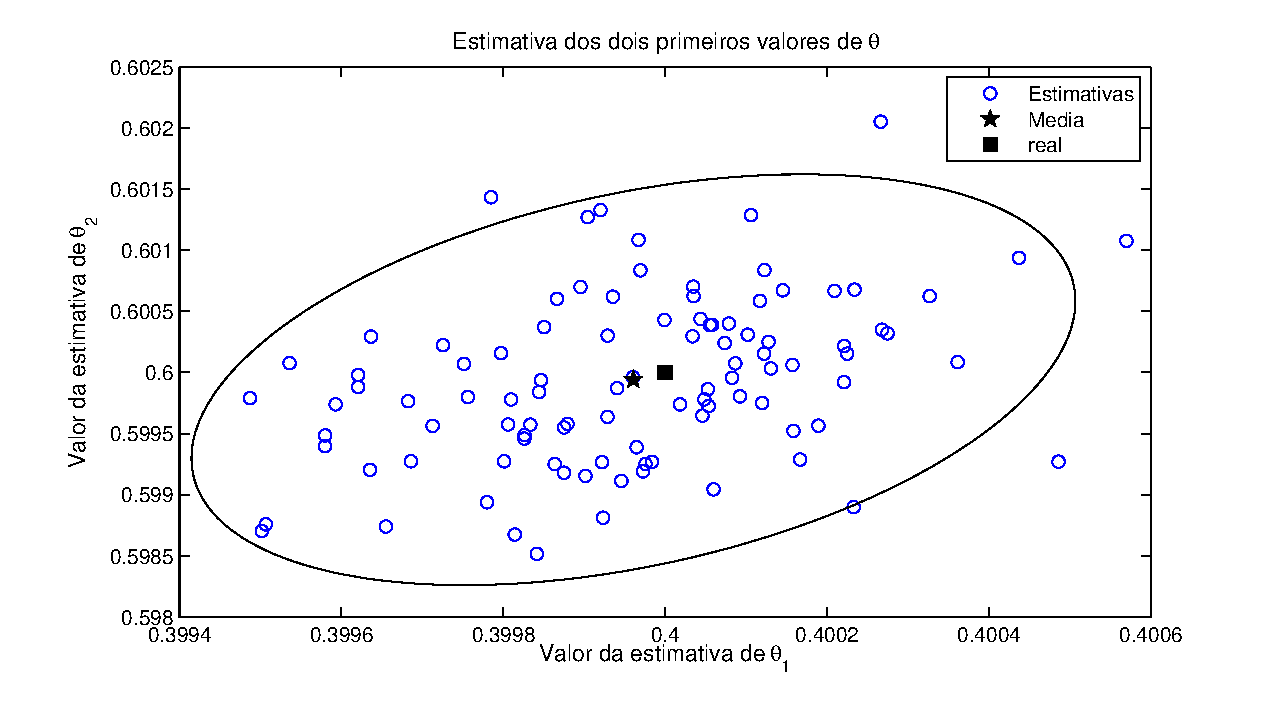
\includegraphics[width=0.95\columnwidth]{figures/vrft_nl_dynamic_t1_t2.eps}
	\caption{100 esperimentos de Monte Carlo das vari�veis $\theta_1$ e $\theta_2$}
	\label{fig:vrft_nl_dynamic_t1_t2}
\end{figure}

O custo $J_{VR}=2.7291\times10{-8}$ foi obtido utilizando-se os sinais de sa�da do controlador obtido e
esperado. J� o custo entre os sinais de sa�da do sistema em malha fechada estimado e desejado foi de
$J_{MR}=0.0033$.

Com o intuito de demonstrar o efeito do ru�do sobre as estimativas obtidas o ruido foi aumentado em $4\times$ para
$\sigma^2 = 0.02$. Obteve-se desta forma os seguintes resultados paras as estimativas:

\begin{equation}
\theta_{\text{m�dia}}=\begin{bmatrix}
0.3999 & 0.5996 & 0.1001 & 0.1502 & 0.4999
\end{bmatrix}
\nonumber
\end{equation}

\begin{equation}
\theta_{\text{Desvio padr�o}}=\begin{bmatrix}
0.0010 & 0.0027 & 0.0012 & 0.0027 & 0.0012
\end{bmatrix}
\nonumber
\end{equation}

\begin{equation}
\theta_{\text{Covari�ncia}}=1.0\times 10^{-5}\begin{bmatrix}
    0.1061 &  0.1207 & -0.0894 & -0.1185 & -0.0310 \\
    0.1207 &  0.7122 & -0.1048 & -0.5357 &  0.0038 \\
   -0.0894 & -0.1048 &  0.1344 &  0.1972 & -0.0033 \\
   -0.1185 & -0.5357 &  0.1972 &  0.7523 & -0.0571 \\ 
   -0.0310 &  0.0038 & -0.0033 & -0.0571 &  0.1355
\end{bmatrix}
\nonumber
\end{equation}

Com os custos de $J_{VR}=1.0326\times10{-7}$ e $J_{MR}=0.0054$, corroborando para o fato de que os custos n�o
foram significativamente afetados pelo aumento do ru�do. Fazendo assim com que a estimativa ainda seja confi�vel.

%===============================================================================
\subsubsection{Controlador ideal sendo representado pela classe de modelos 2}
\label{sec:dbnarmax_nl_dinamic_c_match2}
%===============================================================================

%===============================================================================
\subsubsection{Controlador n�o sendo representado pelo modelo}
\label{sec:dbnarmax_nl_dinamic_c_not_match}
%===============================================================================

Neste exemplo ser� abordado o caso onde o controlador $C(z, \theta) \notin \mathcal{C}$. Fazendo com que o sistema em
malha fechada n�o consiga ter a din�mica esperada. Considere a planta n�o linear descrita por:

\begin{equation}
y(t)=\frac{0.5u(t-1)y(t-1)+u(t-1)}{1+0.25y^2(t-2)}
\label{eq:vrft_nl_dinamic_ex3_y}
\end{equation}

Deseja-se que em malha fechada seu comportamento seja linear como em:

\begin{equation}
M(z)=\frac{0.4}{z-0.6}
\label{eq:vrft_nl_dinamic_ex3_mz}
\end{equation}

A equa��o \eqref{eq:vrft_nl_dinamic_ex3_mz} pode ser reescrita em fun��o do tempo como em:

\begin{equation}
y(t)=0.4r(t-1)+0.6y(t-1)
\label{eq:vrft_nl_dinamic_ex3_mt}
\end{equation}

Ao igualar a equa��o \eqref{eq:vrft_nl_dinamic_ex3_y} com \eqref{eq:vrft_nl_dinamic_ex3_mt} e isolar o
sinal $u(t)$ tem-se a equa��o que descreve o comportamento do controlador que levar� a planta a ter o
comportamento descrito por $M(z)$ em malha fechada. Obt�m-se desta forma um controlador ideal como em:

\begin{equation}
u(t)=\frac{0.4r(t)+0.6y(t)+0.1y^2(t-1)r(t)+0.15y(t)y^2(t-1)}{1+0.5y(t)}
\label{eq:vrft_nl_dinamic_ex3_cd}
\end{equation}

No exemplo apresentado na se��o \ref{sec:dbnarmax_nl_dinamic_c_match} foi apresentada a simula��o para quando o controlador
�timo consegue ser descrito pelo modelo escolhido para representa-lo. Neste exeplo deseja-se o oposto: que a classe de
modelos escolhida para o controlador n�o consiga representar completamente \eqref{eq:vrft_nl_dinamic_ex3_cd}. Para isso
escolheu-se a seguinte classe de modelos para representar o controlador:

\begin{equation}
u(t)=\frac{\theta_1 r(t)+ \theta_2 y(t)+ \theta_3 r(t)y(t-1)+ \theta_4 y(t-1)y(t)}{1+ \theta_5 y(t)}
\label{eq:vrft_nl_dinamic_ex3_c}
\end{equation}

Para as simula��es foi adicionado um ru�do com $\sigma^2 = 0.05$. Foram realizados 100 experimentos de Monte Carlo onde
obteve-se as seguintes estimativas:

\begin{equation}
\theta_{\text{m�dia}}=\begin{bmatrix}
0.4696 & 0.7011 & 0.0083 & 0.0063 & 0.5013
\end{bmatrix}
\label{eq:vr_rational_ex3_theta}
\end{equation}

\begin{equation}
\theta_{\text{Desvio padr�o}}=\begin{bmatrix}
0.0017 & 0.0058 & 0.0020 & 0.0064 & 0.0025
\end{bmatrix}
\nonumber
\end{equation}

\begin{equation}
\theta_{\text{Covari�ncia}}=1.0\times 10^{-4}\begin{bmatrix}
    0.0278 &  0.0396 &  0.0035 &  0.0146 & -0.0137 \\
    0.0396 &  0.3328 &  0.0066 & -0.1651 &  0.0063 \\
    0.0035 &  0.0066 &  0.0382 &  0.0688 & -0.0119 \\
    0.0146 & -0.1651 &  0.0688 &  0.4130 & -0.0562 \\
   -0.0137 &  0.0063 & -0.0119 & -0.0562 &  0.0646
\end{bmatrix}
\nonumber
\end{equation}

Obte-se um custo para o comportamento do sistema em malha fechada de  $J_{MR}=1.0999$. Na Figura
\ref{fig:vr_rational_notinclass_ex3_error} � apresentado o erro para o sistema desejado e o sistema obtido utilizando-se
o modelo obtido com os valores de $\theta$ apresentados em \eqref{eq:vr_rational_ex3_theta} para uma refer�ncia do tipo
degrau unit�rio.

\begin{figure}[htbp] 
	\center 
	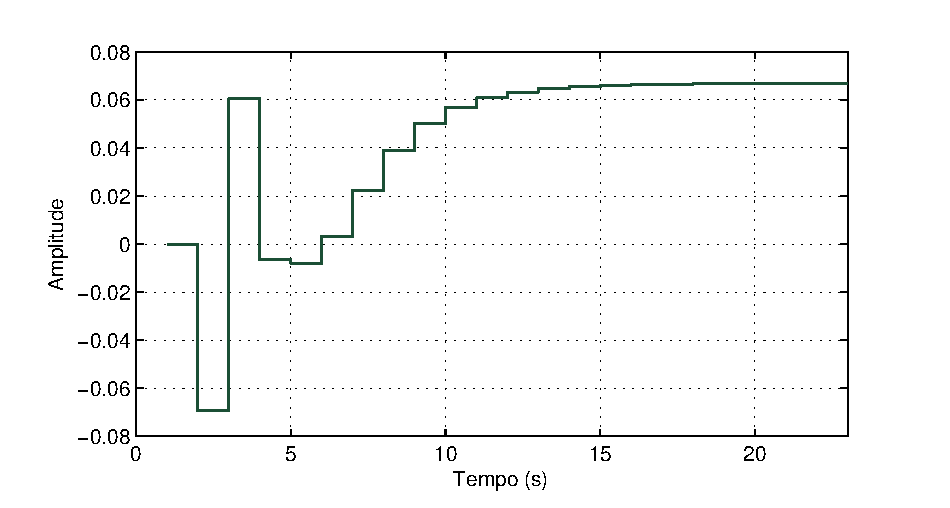
\includegraphics[width=0.95\columnwidth]{figures/vr_rational_notinclass_ex3_error.eps}
	\caption{Erro entre o comportamento do sistema em malha fechada e o comportamento em malha fechada desejado.}
	\label{fig:vr_rational_notinclass_ex3_error}
\end{figure}























%===============================================================================
\section{Considera��es Finais}
\label{sec:dbnarmax_conclusions}
%===============================================================================

Neste cap�tulo apresentou-se a uni�o das ideias de utiliza��o de refer�ncia virtual para a obten��o dos sinais
necess�rios para a determina��o do controlador �timo e a ideia de utiliza��o de algoritmos de identifica��o de sistemas
n�o lineares para determina��o do controlador �timo quando este faz parte de uma classe de modelos n�o linear.

Descreveu-se inicialmente a ideia generalizada onde a classe de modelos n�o linear do controlador precisa estar atrelada
apenas ao algoritmo utilizado para sua identifica��o. Devido aos bons resultados obtidos com a identifica��o de sistemas
NARMAX apresentados no Cap�tulo \ref{chapter:nlin_si_ident}, optou-se por utilizar este algoritmo (Se��o
\ref{sec:nl_si_algorithms_rationals}) para determinar os par�metros do controlador utilizando-se para isso entretanto
dos sinais obtidos por meio do m�todo de refer�ncia virtual.

Nas Se��es \ref{sec:dbnarmax_wiener_hammerstein} e \ref{sec:dbnarmax_rational_controllers} apresentou-se alguns
exemplos para demonstrar a viabilidade da utiliza��o da metodologia. Foram apresentados exemplos onde a classe de
modelos consegue representar a totalidade das din�micas de $\mathcal{C}_d$ para que o sistema se comporte em malha
fechada linearmente como escolhido por $T_d(z)$. Outro exemplo foi apresentado quando n�o existe uma completa descri��o
do controlador ideal pela classe de modelos, ou seja, $\mathcal{C}_d \notin \mathcal{C}$, apresentou-se um comparativo
do sistema ideal e do obtido utilizando o controlador obtido quando o sistema � submetido a um degrau unit�rio.

Tamb�m foi apresentado um exemplo onde o controlador � descrito por um modelo NARMAX polinomial, em um contexto onde a
planta do sistema possui uma n�o linearidade est�tica na sa�da do processo, caso este onde o controlador ideal tamb�m
n�o se encontra na classe de modelos. A aproxima��o do modelo escolhido para este controlador se mostrou relativamente
pr�ximo ao controlador ideal, visto que o cancelamento da n�o linearidade da planta foi quase completo, como apresentado
na Figura \ref{fig:vrft_nl_wiener_vw}.

De forma geral, apresentou-se neste cap�tulo a utiliza��o desta metodologia de identifica��o de controladores n�o
lineares descritos por modelos NARMAX, polinomial ou racional e seus resultados. Os resultados obtidos mostram que a
metodologia � v�lida e que em situa��es onde o controlador ideal pode ser bem representado pela classe de controladores,
os resultados obtidos n�o possuem erro de polariza��o para experimentos executados em malha aberta. 

%===============================================================================
